%%%%%%%%%%%%%%%%%%%%%%%%%%%%%%%%%%%%%%%%%%%%%%%%%%%%%%%%%%%%%%%%%%%%%%%
% TCC 1 - Engenharia de Software
% Autores: Henrique Alberone e Mateus Fonseca
% Professores: Laerte Xavier e Lesandro Ponciano
%%%%%%%%%%%%%%%%%%%%%%%%%%%%%%%%%%%%%%%%%%%%%%%%%%%%%%%%%%%%%%%%%%%%%%

\documentclass[12pt]{article}
\usepackage{sbc-template}
\usepackage{graphicx,url}
\usepackage{float} 
\usepackage[brazil]{babel}
\usepackage{tabularx}
\newcolumntype{C}{>{\centering\arraybackslash}X} % <-- modified
\usepackage[utf8]{inputenc}  
\usepackage[inline]{enumitem}
\usepackage{tcolorbox}

\sloppy

\title{Estudo sobre a técnica de modelagem de usuário \emph{persona} e suas dificuldades de aplicação}

%\title{Estudo sobre a técnica de criação de \emph{personas} e as dificuldades de sua aplicação}
%\title{Estudo sobre \emph{personas} e sua dificuldade em representar precisamente os usuários de um sistema}
%\title{Estudo sobre a precisão da técnica de criação de \emph{personas}}
%\title{Estudo sobre personas e sua dificuldade em representar todos os usuários de um sistema - Titulo Provisório}%

\author{Henrique Alberone Nunes Alves Ramos\inst{1}, Mateus Santos Fonseca\inst{1} }

\address{Bacharelado em Engenharia de Software\\Instituto de Ciências Exatas e Informática – PUC Minas\\Rua Cláudio Manoel, 1162, Funcionários, Belo Horizonte – MG – Brasil\linebreak
 \email{\{hanaramos, mateus.fonseca.1092523\}@sga.pucminas.br}
}

%2-3 linhas contextualização, 2-3 linhas problema, 2 linhas objetivo, 3 linhas metodologia e o que vamos entregar de resultado

\begin{document} 

\maketitle

\begin{abstract}
  \par User modeling is a technique that aims to represent a conceptual user for a product, whether it is a system or not. This technique is frequently used by designers who aim to improve the user experience. In its creation process, information about the target audience can be lost if they deviate from the ``standard", making the result less comprehensive. This work aims to analyze the techniques of user modeling, especially the technique of creating personas, through a pure descriptive research, seeking to understand the reasons why nonstandard users aren't being represented.
  \vskip0.1in
  \par \textbf{Keywords:} \emph{user experience, user modeling, persona, user profile, empathy map, human-computer interaction}
  

\end{abstract}
     
\begin{resumo} 
    \par Modelagem de usuário é uma técnica que tem como finalidade representar um usuário conceitual para um produto, seja ele um sistema ou não. Essa técnica é recorrentemente utilizada por projetistas que almejam melhorar a experiência do usuário. Em seu processo de criação, informações a respeito do público-alvo podem se perder caso destoem do ``padrão", tornando o resultado menos abrangente. Este trabalho almeja analisar a de modelagem de usuário persona, por meio de uma pesquisa descritiva pura, buscando compreender os motivos que fazem usuários ``fora da curva" não serem representados.
    \vskip0.1in
    \par \textbf{Palavras chave:} \emph{experiência de usuário, modelagem de usuário, persona, perfil do usuário, mapa de empatia, interação humano-computador}
\end{resumo}

\begin{tcolorbox}
\footnotesize
\textbf{Bacharelado em Engenharia de \emph{Software} - PUC Minas\\
Trabalho de Conclusão de Curso (TCC)} \\

\indent Orientador de conteúdo (TCC I): Laerte Xavier - laertexavier@gmail.com\\
Orientador acadêmico (TCC I): Lesandro Ponciano - lesandrop@pucminas.br\\
Orientador do TCC II: Lesandro Ponciano - lesandrop@pucminas.br\\ \\
Belo Horizonte, 15 de novembro de 2020.
\end{tcolorbox}

\section{Introdução} \label{sec:introducao}
\emph{User Experience} (UX) é um tópico recorrente na área de Engenharia de \emph{Software}. Este conceito está diretamente conectado na capacidade de um produto, seja ele um sistema ou não, em proporcionar boas sensações aos usuários \cite{10.1145/3357155.3358444}. Com esta finalidade, \emph{UX designers} buscam modelar os usuários do sistema. Para isto, uma das técnicas utilizadas é a construção de \emph{personas}. \emph{Personas} são representações de potenciais clientes ou usuários por meio de uma pessoa imaginária, normalmente com uma foto e descrita por um conteúdo textual \cite{10.1145/3265986}. Além disso, elas também representam usuários arquetípicos e incorporam suas necessidades e objetivos \cite{10.1145/1978942.1979274}. 

\par As \emph{personas} são modelos de usuários criados a partir de uma síntese dos resultados de uma pesquisa realizada com um público-alvo. Este modelo auxilia na elicitação de requisitos de forma ágil e em desenvolver uma experiência de uso agradável ao público \cite{10.1145/3274192.3274210}. A melhora no planejamento e desenvolvimento de um produto é evidente ao utilizá-las, pois fornecem um foco aos \emph{designers} que possuem ideias vagas ou contraditórias sobre quem são seus usuários \cite{10.1145/3027063.3053355}. No entanto, sua utilização pode excluir parte dos usuários que não se comportem como os poucos grupos modelados como \emph{personas}, ocasionando em um projeto não-inclusivo da interface do \emph{software}.

\par Neste contexto, o problema investigado neste estudo é a dificuldade em representar os usuários de um sistema ou produto que estejam fora do padrão, através da modelagem de \emph{personas}. Tendo em vista a necessidade de melhorar a satisfação dos usuários, mostra-se relevante a realização de um estudo aprofundado acerca das dificuldades na aplicação das técnicas de modelagem de \emph{personas}. Essa importância se dá por meio da definição e descrição dos potenciais usuários do sistema, uma vez que essa modelagem auxilia os desenvolvedores e \emph{designers} a estimular sentimentos positivos das pessoas ao interagirem com o \emph{software}.

\par O objetivo geral deste artigo é analisar as técnicas de modelagem de \emph{personas}, buscando compreender os motivos que fazem usuários fora do padrão não se sentirem representados. Para atingir esse objetivo, são propostos os seguintes objetivos específicos: 
\begin{enumerate*}[label=\roman*)]
    \item Identificar potenciais dificuldades na criação dos modelos de \emph{personas};
    \item Validar com os usuários a fidedignidade de \emph{personas} criadas com técnicas de modelagem diferentes;
    \item Comparar as técnicas de modelagem de \emph{personas} no que tange ao quesito de precisão na representação dos usuários.
\end{enumerate*}

\par Este trabalho está organizado da seguinte forma: a seção 2 aborda a fundamentação teórica, explorando os conceitos e teorias aplicadas. A seção 3 apresenta os trabalhos relacionados ao estudo e a seção 4 abrange a metodologia utilizada.

\section{Fundamentação Teórica} \label{sec:fundamentacao}
\par Nesta seção, são detalhados os principais conceitos e técnicas que estão envolvidos na solução do problema apresentado. São eles: \emph{UX Design}, modelagem de usuários e técnicas para criação de \emph{personas}.

\subsection{\emph{UX Design}}
\emph UX é definida pela ISO 9241-210 como ``a percepção e resposta de uma pessoa ao uso de um produto, sistema ou serviço"\cite{ISO9241210}. Além de apenas fatores funcionais ou estéticos \cite{Elements_UCD}, é um conceito que auxilia na criação de um bom \emph{software}, uma vez que uma boa experiência de uso leva à fidelização dos usuários. O \emph{design} de uma interface se baseia fortemente na noção de abordar as necessidades do usuário relacionadas à interação \cite{Hassenzahl} \cite{10.1145/2994310.2994356}. Enfim, sabe-se que, para oferecer uma experiência ao usuário de alta qualidade, é necessário que sejam orquestrados todos os aspectos da experiência do usuário, o que é difícil, pois o público está em constante mudança \cite{10.1145/1060189.1060209} \cite{10.1145/1512714.1512717}. 

\subsection{Modelagem de usuários}
Modelos de usuários são representações de propriedades de um indivíduo, incluindo necessidades, preferências e características, físicas, cognitivas e comportamentais \cite{mohamad_kouroupetroglou}. Entre as técnicas utilizadas para a modelagem estão: Mapa de Empatia, Perfil do Usuário e \emph{personas}.

\subsubsection{Mapa de Empatia}
\par Mapa de Empatia é uma técnica de modelagem de usuário que favorece a melhor compreensão do contexto do usuário representado a partir de 6 variáveis a serem consideradas: o que ele diz, faz, vê, ouve, sente e pensa. Além dessas, há também as áreas de dores e necessidades, conforme representado na Figura \ref{fig:MapaEmpatia} \cite{gasca2014}. Essa técnica ultrapassa características demográficas e busca compreender o ambiente, os comportamentos, as aspirações e as preocupações do cliente \cite{7328012}. Com esse contexto, pode-se afirmar que um Mapa de Empatia é normalmente utilizado almejando criar empatia com o usuário e aumentar sua satisfação \cite{10.1145/3151470.3156642}. Outra característica do Mapa de Empatia é a sua facilidade em ser adaptado para outros objetivos, como por exemplo, auxiliar a criação de \emph{personas} \cite{7328012}.

\begin{figure}[H]
    \centering
    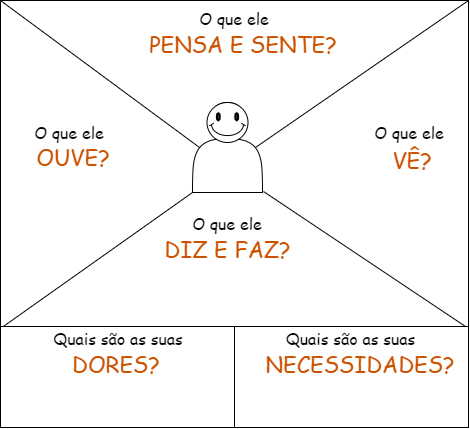
\includegraphics[width=0.6\textwidth]{images/Mapa_Empatia.png}
    \caption{Exemplo de um \emph{template} de Mapa de Empatia.}
    \label{fig:MapaEmpatia}
\end{figure}

\subsubsection{Perfil do Usuário}
\par No contexto de modelagem de usuários, \emph{designers} definem a técnica de Perfil do Usuário como um resumo biográfico fictício, com a adição de objetivos e personalidades \cite{10.1007/BF00143964}. Através da coleta dos dados dos usuários, seja por métodos quantitativos ou qualitativos, é possível agregar os valores em grupos e faixas onde os usuários se encaixam e traçar os perfis de usuários com características similares bem como calcular a proporção de usuários que se encaixam em cada perfil \cite{barbosa2010interacao}.

Portanto essa técnica permite representar o contexto e preferências dos usuários como um conjunto de conceitos e compreender as diferenças genéricas entre grupos de usuários que partilham características semelhantes. Após compreender essas diferenças, torna-se possível, por meio da aplicação de recomendações de usabilidade adequadas ao grupo populacional abordado, uma melhor definição da interface \cite{10.1145/1111360.1111388} \cite{7358378}.

\begin{figure}[H]
    \centering
    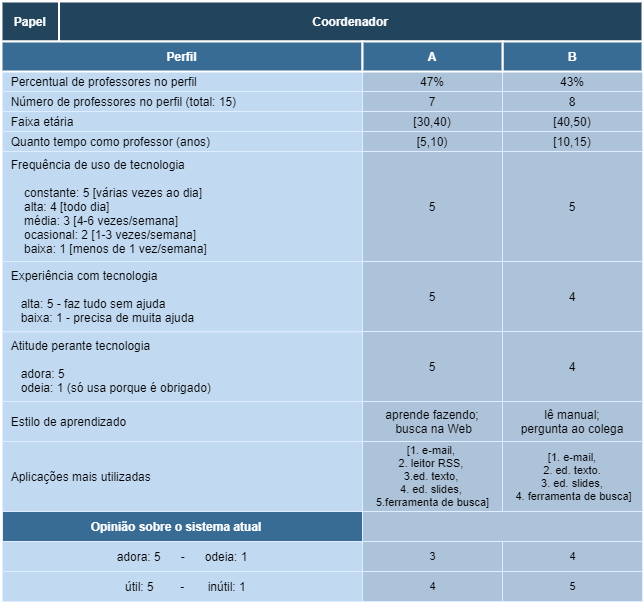
\includegraphics[width=0.882\textwidth]{images/PerfilDoUsuario.png}
    \caption{Exemplo de um Perfil de Usuário de coordenadores de curso}
    \label{fig:PerfilDoUsuario}
    {Fonte: Barbosa e Silva (2010).}
\end{figure}

\subsubsection{\emph{Personas}}
Para desenvolver um sistema agradável ao seus usuários, é necessário entendê-los. Para tanto, faz-se necessário pensar em formas de modelar os usuários. A utilização de \emph{personas} auxilia essa tarefa. \emph{Personas} são personagens fictícios criados para representar o usuário alvo, conforme apresentado na Figura \ref{fig:persona} \cite{Book_Universal_Principles_Design}. Sua criação e utilização é pertinente no \emph{User-Centered Design} (UCD), uma abordagem de desenvolvimento na qual o usuário deve ser pensado e compreendido durante todo processo de concepção, desenvolvimento e implementação do produto \cite{5529821}.  
\par Portanto, dado este contexto, é possível afirmar que \emph{personas} ajudam os \emph{designers} a terem uma visão mais concreta de quem são os seus usuários, em vez de uma visão abstrata \cite{10.5555/1076976}. Além disso, elas fazem com que os desenvolvedores do produto criem empatia pelas pessoas representadas \cite{10.5555/553473}. No entanto, os resultados empíricos da aplicação desta técnica são criticados, sendo argumentado que as \emph{personas} não podem ser consideradas descrições de usuários reais \cite{10.1177/154193120605000503}. Porém, embora seu uso seja criticado em alguns aspectos, estudos indicam que equipes de \emph{design} orientadas por elas podem ser mais produtivas e comunicativas, gerando produtos cujos atributos de usabilidade são melhores para os usuários \cite{long_study}.

\begin{figure}[H]
    \centering
    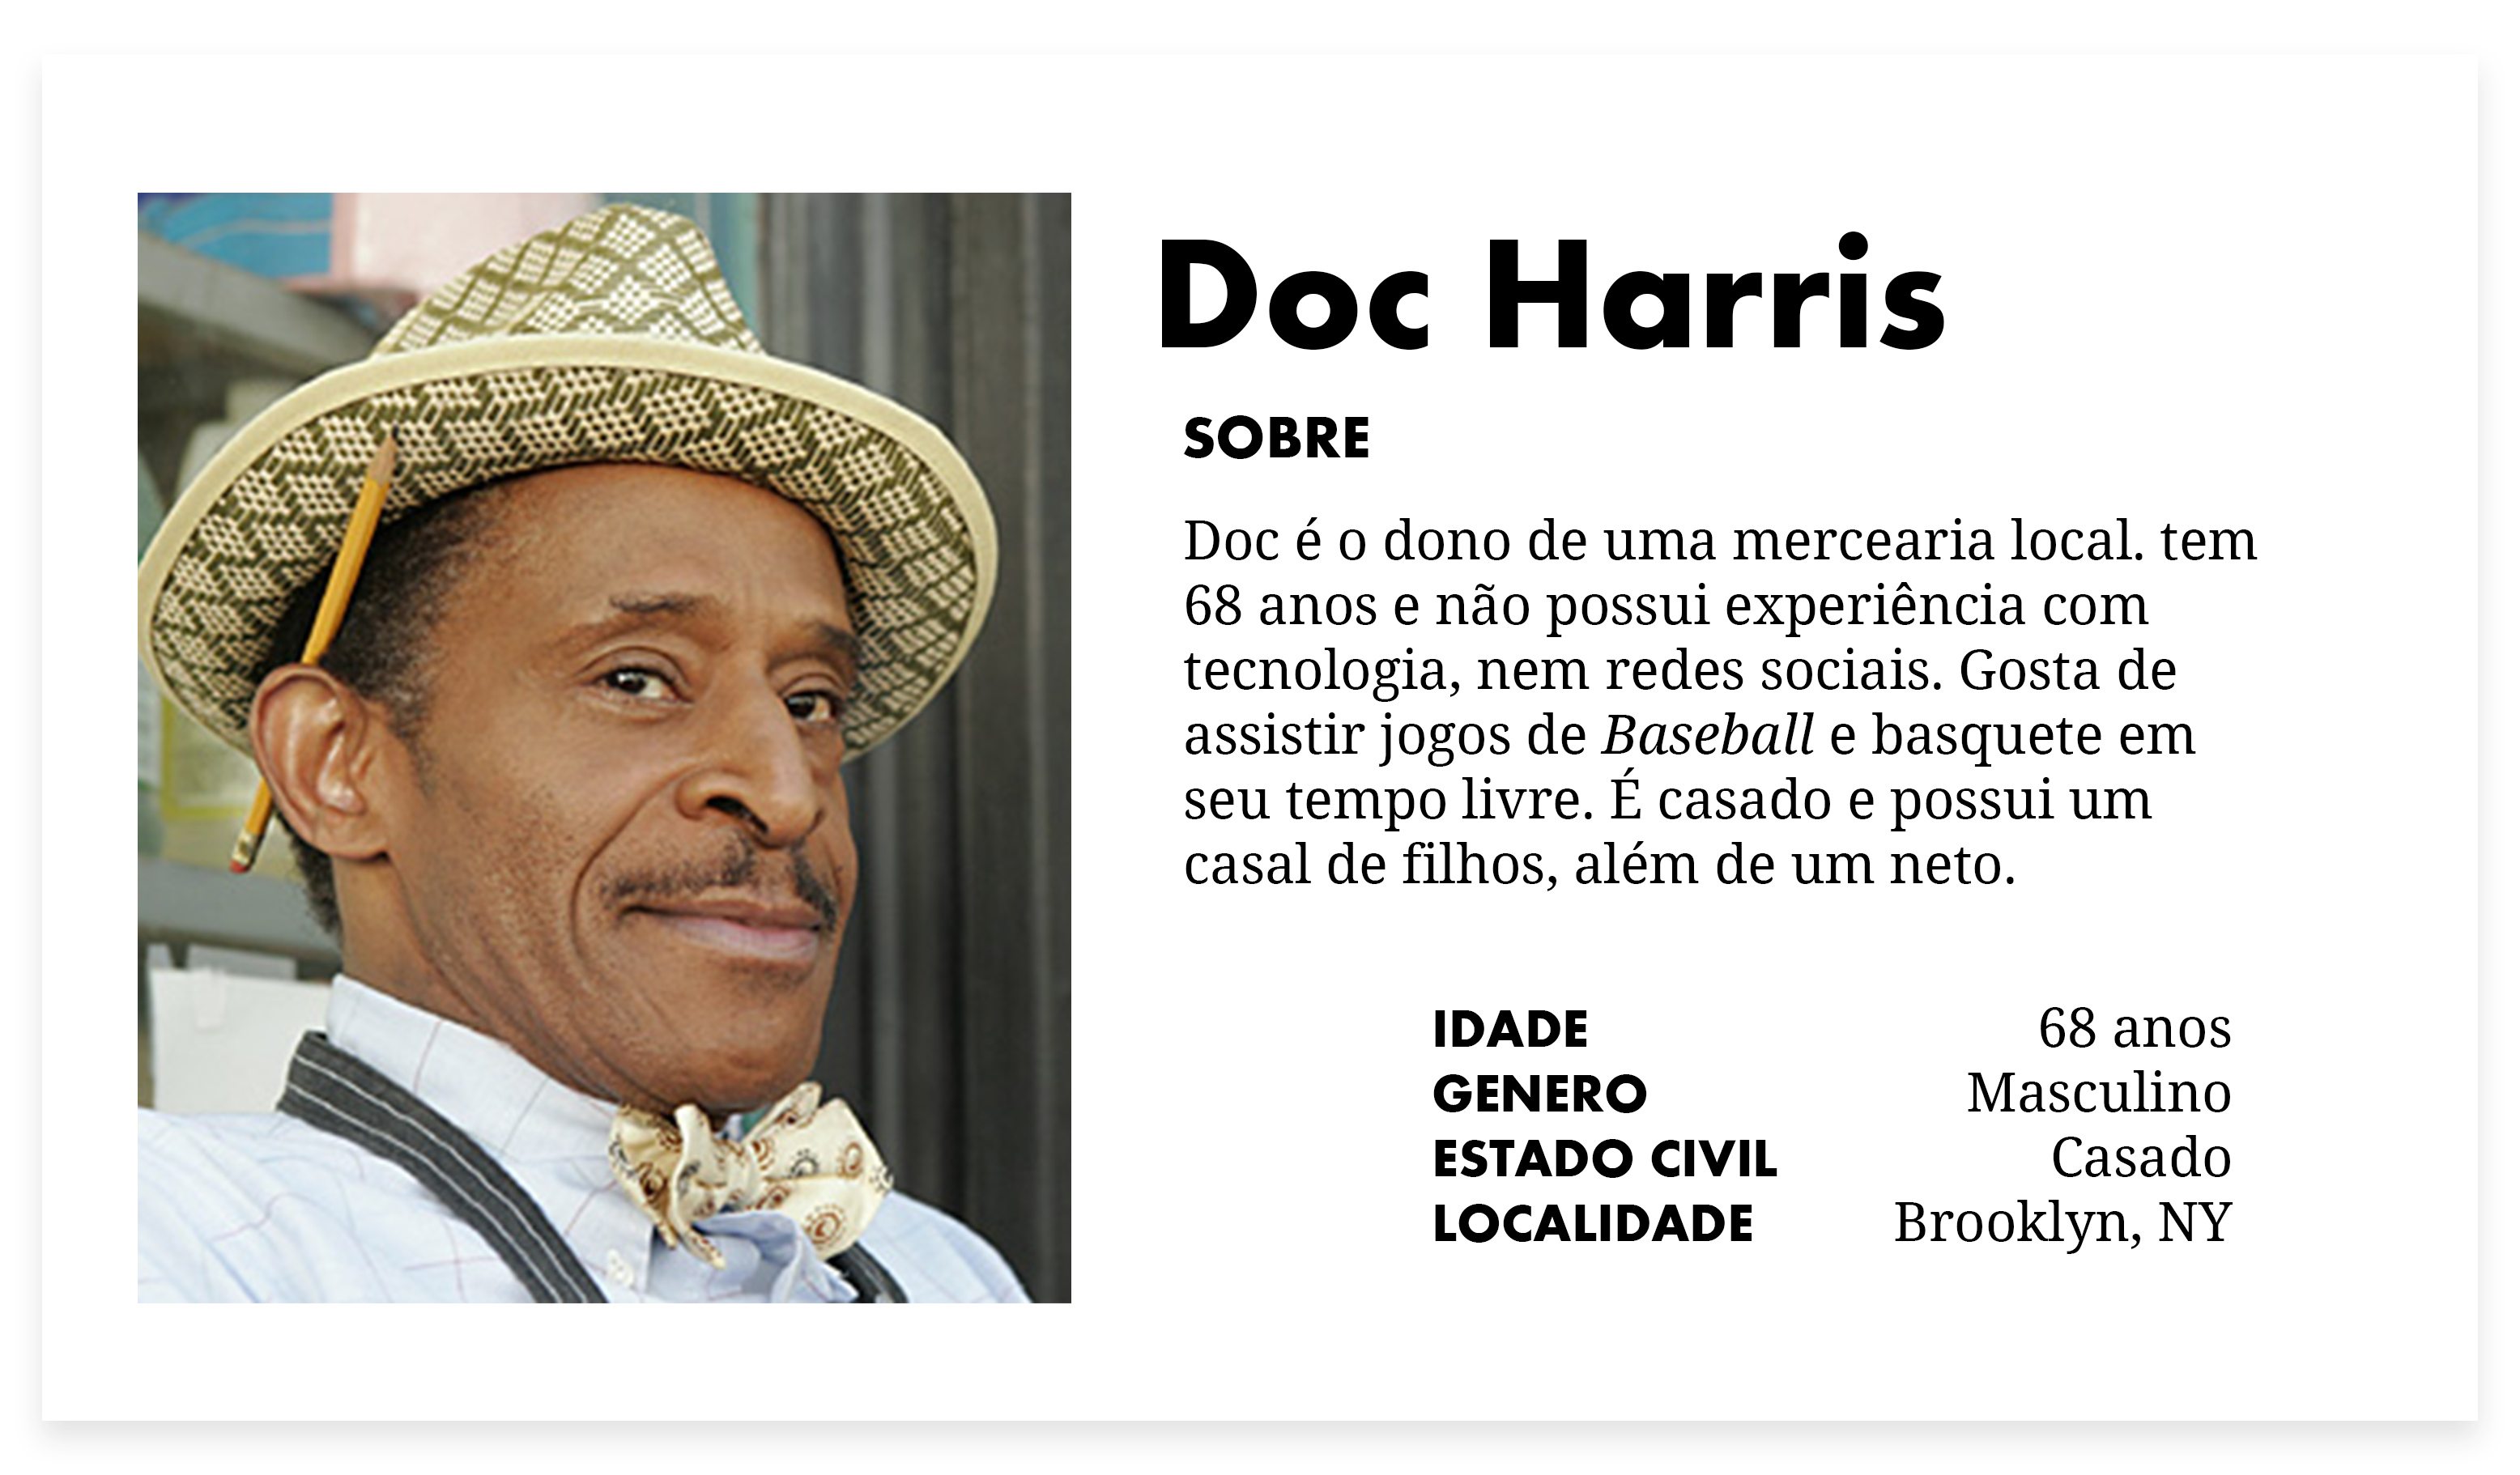
\includegraphics[width=0.795\textwidth]{images/persona.png}
    \caption{Exemplo de uma \emph{Persona}.}
    \label{fig:persona}
\end{figure}

\subsection{Técnicas de criação de \emph{personas}}
Técnicas quantitativas, como aplicação e coleta de resultados de questionários, e técnicas qualitativas, como entrevistas, pesquisas de campo e até mesmo a utilização de outros modelos como Mapa de Empatia e Perfil do Usuário para auxiliar a fornecer dados qualitativos, são as principais formas de obtenção de dados para a criação de \emph{personas} \cite{5928355}. A disposição de tempo e recursos é um fator determinante na escolha do método de coletas de informações e podendo, inclusive, ser puramente quantitativo ou qualitativo, o que não é preconizado na literatura de Interação Humano-Computador (IHC) \cite{10.1145/997078.997089} \cite{10.1007/978-3-642-03658-3_56}. Com a aplicação desses métodos, as informações obtidas possibilitam fazer, com maior precisão, o detalhamento das características do usuário, que serve de insumo para o desenvolvimento de uma \emph{persona} \cite{7328012}.

\par Uma \emph{persona} também pode ser construída baseada em outros modelos como, por exemplo, um Mapa de Empatia. Baseado nesse artefato, o \emph{UX Designer} é capaz de compreender o contexto no qual o usuário está inserido e, de forma empática, analisar suas necessidades, preocupações e aspirações \cite{7328012}. Finalmente, deve-se analisar as muitas informações obtidas, uma vez que elas podem não ser relevantes para o processo de desenvolvimento do produto. Portanto, essas informações devem ser filtradas para que as \emph{personas} não contenham conteúdo desnecessário, tendo em vista que a ausência de foco pode atrapalhar o desenvolvimento do produto \cite{7328012}.

\section{Trabalhos Relacionados} \label{sec:trabalhosrelacionados}
Os trabalhos relacionados discutidos neste artigo envolvem estudos acerca de UX \cite{10.1145/3357155.3358444}. Além de abordar de forma geral UX, os estudos nesta seção aprofundam em um conceito fundamental do UX: as técnicas de modelagem de usuários, sendo abordadas as técnicas de \emph{persona}, Mapa de Empatia e Perfil do Usuário \cite{long_study} \cite{7328012} \cite{10.1145/3313831.3376502} \cite{10.1007/978-3-642-03658-3_56}.

\par Em uma tentativa de entender o que a comunidade acadêmica brasileira entende por \emph{User Experience}, bem como o seu conceito e escopo, os autores Melo e Darin (2019) propõem uma pesquisa em uma plataforma \emph{on-line} entre profissionais, acadêmicos ou de mercado, envolvidos com IHC \cite{10.1145/3357155.3358444}. Nessa plataforma, foi disponibilizada uma \emph{survey}, no mesmo modelo proposto por Law et al. \cite{10.1145/1518701.1518813}, que continha três seções: Declarações sobre UX, Definições de UX e Informações Gerais. Através dos dados obtidos, como resultado, evidenciou-se uma diferença significativa entre a definição de UX na comunidade nacional em contraste com a internacional. Esse estudo é relevante para nosso trabalho devido à análise do conceito de UX, principalmente, no Brasil. Além disso, esse artigo evidencia a necessidade de se aprofundar no conhecimento de UX em diversos tópicos, o que inclui as técnicas de modelagem de usuários.

\par Embora o uso de \emph{personas} em ambientes de \emph{design} colaborativo esteja bem estabelecido, poucas pesquisas foram realizadas para quantificar os benefícios do uso desta técnica \cite{long_study}. Com esse contexto, Long (2009) propõe um experimento que busca investigar a eficácia de \emph{personas} e as vantagens de sua aplicação na criação de soluções mais eficazes e centradas no usuário. O experimento foi planejado como um projeto de \emph{design} e conduzido durante um período de cinco semanas por três grupos compostos por alunos do 3º ano de Design Industrial. Os resultados indicaram que os grupos de alunos que utilizaram \emph{personas} produziram produtos com características de usabilidade superiores. Os resultados mostraram também que o uso de \emph{personas} fornece uma vantagem significativa durante os estágios de pesquisa e conceituação do processo de \emph{design}. O fato desse estudo evidenciar as vantagens que a utilização de \emph{personas} podem trazer para o UX dos usuários de um sistema o torna apropriado para ser avaliado no estudo atual.

\par Em seu artigo, Ferreira et al. (2015) afirmam que considerar as necessidades e emoções dos usuários é essencial no sucesso de um produto de \emph{software} \cite{7328012}. Neste contexto, visando auxiliar os profissionais a projetar para os usuários e tornar as \emph{personas} mais direcionadas para a aplicação sem perder o foco no usuário, os autores criaram a técnica PATHY (\emph{Personas} \emph{empATHY}). Essa técnica integra as perguntas-guia e a estrutura do Mapa de Empatia com a ideia de descrever usuários por meio de \emph{personas}. As \emph{personas} geradas pela técnica evidenciaram que algumas perguntas-guia influenciam na qualidade dos requisitos gerados e, além disso, geram dados relevantes para conhecer melhor o usuário. A importância desse artigo se dá na relação direta criada entre a técnica de \emph{personas} e Mapa de Empatia. Além disso, embora não seja explícito no artigo, fica evidente que \emph{personas} podem ser, algumas vezes, imprecisas.

\par No estudo realizado por Salminen et al. (2020)\cite{10.1145/3313831.3376502}, são enfatizados os vários benefícios da criação de \emph{personas}. Porém, é ponderado pelos autores que a criá-las utilizando métodos qualitativos pode não ser preciso o suficiente. Para sanar esses problemas de precisão, os autores indicam a utilização de dados quantitativos, pois seu uso auxilia a construção de arquétipos de usuário mais precisos e atraentes. Entretanto, é apontado pelos autores a falta de uma visão geral sistemática dos métodos de criação quantitativa de \emph{personas} (CQP) e, abordando essa lacuna, é realizada uma revisão de 49 artigos de CQP. Os resultados indicam que o compartilhamento de recursos como \emph{datasets}, códigos e algoritmos é crucial para atingir a maturidade do CQP. Esse artigo é relevante para nossa pesquisa, uma vez que ele aborda a criação de \emph{personas}, evidencia a imprecisão dos métodos qualitativos e apresenta as dificuldades existentes na construção de \emph{personas} por meio de métodos quantitativos.

\par Em seu estudo, Thoma e Williams (2009) buscam melhorar a criação de \emph{personas}, apontando problemas na escolha de métodos, nos procedimentos e em sua validação \cite{10.1007/978-3-642-03658-3_56}. Para aperfeiçoar esta modelagem, os autores propõem uma abordagem heurística, envolvendo métodos qualitativos e quantitativos, visando obter um resultado mais preciso. Dentre os resultados obtidos nesse artigo, o principal é a validação dos métodos de criação de \emph{persona}. Além disso há a constatação da importância de se utilizar métodos quantitativos e qualitativos juntos para obter dados que servem de insumo para modelar os usuários. Tendo em vista que esse trabalho busca, também, melhorar as técnicas de modelagem de usuários, ele mostra-se valioso para nosso estudo, uma vez que nosso estudo busca atenuar a exclusão de clientes que estejam fora da curva.

\section{Materiais e Métodos} \label{sec:materiaisemetodos}
Este estudo se trata de uma pesquisa descritiva pura quantitativa e qualitativa. O objetivo de uma pesquisa descritiva é descrever um fenômeno e suas características \cite{10.1177/1362168815572747}. Dessa forma, a presente pesquisa é classificada como descritiva pois, por meio de diversas análises, busca-se descrever \emph{personas}, compará-las e sugerir melhorias para os respectivos processos de criação.

Além disso, sabe-se que uma pesquisa pura tem como objetivo a busca em melhorar as teorias científicas para melhor compreensão e previsão de fenômenos \cite{1954-06834-000}. Neste contexto, nossa pesquisa classifica-se como pura pois busca compreender os motivos pelos quais \emph{personas} podem ter imprecisões na representação de usuários. 

\par Finalmente, esta pesquisa é classificada como quantitativa no que tange aos resultados obtidos por meio da aplicação dos questionários aos participantes, nos quais é possível quantificar a precisão em representar o usuário de cada modelo projetado. Além disso, o presente estudo também é classificado como qualitativo devido aos resultados da aplicação de um questionário qualitativo aos \emph{designers} dos modelos de usuários. Esse questionário almeja identificar possíveis dificuldades na utilização das técnicas de criação de \emph{personas} dentro do contexto de um domínio de sistema específico.

\par Tendo as \emph{personas} como objeto de estudo, este trabalho busca analisar a precisão desta técnica de modelagem de usuários, em relação a representação dos usuários. A seção a seguir contempla as etapas necessárias para a realização deste estudo, assim como os procedimentos e o cronograma das atividades.

\subsection{Procedimentos}
\par É proposto no presente trabalho a verificação dos motivos pelos quais as \emph{personas} podem ser imprecisas na tentativa de representar os usuários. Além disso, este estudo também busca realizar uma comparação, visando analisar a precisão de 3 \emph{personas} criadas através de técnicas diferentes: 
\begin{enumerate*}[label=\roman*)]
    \item \emph{personas};
    \item \emph{personas} baseadas em Mapa de Empatia;
    \item \emph{personas} baseados em Perfil do Usuário.
\end{enumerate*} 

Para o desenvolvimento deste estudo, são utilizados métodos quantitativos e qualitativos na obtenção de dados dos usuários. A escolha da utilização de ambos os métodos é baseada na proposição de que a utilização combinada de métodos auxilia a construção de arquétipos de usuário mais precisos e atraentes \cite{10.1145/3313831.3376502}.
       
\par A pesquisa foi feita no contexto de analisar a explicabilidade de um software. A escolha desse domínio deve-se a relevância de compreender a percepção dos usuários em relação a importância deste requisito, buscando fazer as seguintes questões
\begin{enumerate*}
    \item 
\end{enumerate*}
, que é 

\par Com o contexto definido, a presente pesquisa é realizada com o total de 30 pessoas, uma vez que um número maior de participantes pode inviabilizar o trabalho devido às dificuldades de conseguir voluntários que estejam dispostos a contribuir efetivamente na pesquisa. A escolha dos participantes se dá por meio de uma amostragem não probabilística, onde o único filtro é justamente que os participantes sejam usuários de sistemas que pertençam ao contexto definido. O método de amostragem utilizado chama-se Amostragem Exponencial Discriminativa em Bola de Neve, onde os participantes inicialmente selecionados indicam outros candidatos até que o número almejado seja alcançado \cite{snow_ball_prob}. O método de comunicação utilizado com todos participantes será o \emph{WhatsApp}, devido a sua facilidade de utilização e por permitir uma comunicação tanto síncrona quanto assíncrona.
       
\par Para iniciar a etapa de obtenção de dados dos usuários, os participantes são submetidos a um questionário qualitativo. É importante frisar que todos os questionários presentes neste estudo são elaborados no \emph{Google Forms}. Neste primeiro questionário, são abordadas as seguintes questões:
\par Questionário 1:
\begin{enumerate}\setlength\itemsep{0.5em}
    \item Qual a sua idade?
    \item Qual o seu gênero?
    \item Qual a sua escolaridade?
    \item Qual a sua profissão atual?
    \item Qual a sua Nacionalidade?
    \item Onde você reside atualmente (cidade e estado)? 
    \item Qual o seu estado civil?
    \item Você possui filhos? Se sim, quantos?
    \item Você utiliza plataformas de jogos com muita frequência?
    \item O que mais te atrai em uma plataforma de jogos?
    \item O que mais te incomoda na utilização de uma plataforma de jogos?
    \item Quantas horas você estima gastar na utilização de uma plataforma de jogos por dia?
    \item Há quanto tempo você utiliza plataformas de jogos?
    \item Quantas plataformas diferentes já utilizou?
\end{enumerate}
       
Essas informações são necessárias para se ter uma ideia inicial das características do participante bem como compreendê-lo como usuário de plataforma de jogos. Visando complementar o questionário, também é realizado com o participante uma entrevista semiestruturada. Essa entrevista busca obter dados relevantes e pessoais dos usuários que o questionário não aborda. Neste roteiro, são definidos os tópicos-chave:
\par Roteiro de entrevista 1:
\begin{enumerate}\setlength\itemsep{0.5em}
    \item Quais são seus \emph{hobbies}?
    \item O que faz no dia a dia?
    \item O que a motiva?
    \item Em termos de personalidade, como o entrevistado se define?
    \item Quais são as categorias de jogos que você mais gosta?
\end{enumerate}
       
Após a obtenção dos dados, as informações coletadas se tornam insumo para o desenvolvimento dos modelos de usuários. Nesta etapa, é realizada a criação dos modelos de usuários pelos autores desta pesquisa, portanto os dados dos usuários mais pertinentes coletados se tornam características dos modelos desenvolvidos. As técnicas de modelagem de usuário utilizadas são a criação de:
\begin{enumerate*}[label=\roman*)]
    \item \emph{persona};
    \item Mapa de Empatia;
    \item Perfil do Usuário.
    \item \emph{persona} baseada em Mapa de Empatia;
    \item \emph{persona} baseada em Perfil do Usuário;
\end{enumerate*}

Durante o processo de construção dos modelos, após cada modelo de usuário construído, o \emph{designer} deve responder a um questionário qualitativo que busca identificar quaisquer dificuldades ao utilizar as técnicas de modelagem de usuário para criação dos modelos. Os resultados deste questionário possibilitam identificar possíveis gargalos e obstáculos pertinentes no processo de criação. O questionário respondido pelo \emph{designer} contempla as seguintes questões: 
\par Questionário 2:
\begin{enumerate}\setlength\itemsep{0.5em}
    \item Você teve alguma dificuldade no processo de criação do modelo?
    \item Você sentiu falta de informações dos usuários para a construção do modelo? Se sim, quais?
    \item Quanto tempo demorou para criar o modelo?
    \item Qual sua opinião, como \emph{designer}, a respeito da técnica utilizada para modelar o usuário?
\end{enumerate} 
       
Com os modelos de usuários projetados, um pequeno questionário quantitativo é utilizado. Esse questionário segue o modelo de respostas em escala \emph{Likert}, no qual as pessoas submetidas são solicitadas a mostrar seu nível de concordância (de discordo totalmente a concordo totalmente) com cada item \cite{likert_scale}. Esse questionário busca receber \emph{feedback} do usuário sobre o quão representado ele se sentiu ao analisar o modelo de usuário. Para isso, são respondidas as seguintes questões: 
\par Questionário 3:
\begin{enumerate}\setlength\itemsep{0.5em}
        \item No geral, consigo me identificar com o modelo apresentado;
        \item Eu me sinto representado pelas características do modelo apresentado;
        \item Um produto que seguir essas características me trará mais satisfação.
\end{enumerate}
Para responder o questionário 3, cada participante visualiza todos os 5 modelos de usuários projetados. Não há limite de tempo para o participante analisar cada modelo, uma vez que é fundamental que ele seja capaz de verificar o quão representado ele foi pelo modelo demonstrado. Logo após a análise de cada modelo, o participante responde ao questionário.

Finalmente, com os resultados obtidos da aplicação dos questionários aos participantes, é possível realizar uma medição que analisa a precisão de cada modelo no que tange à sua capacidade em representar usuários. Para tanto, para cada participante, basta somar a pontuação das respostas dos questionários de cada modelo. Ao final, cada modelo terá a sua pontuação total e, no contexto deste estudo, torna-se possível verificar qual modelo foi mais preciso em relação aos outros.
        
Além disso, uma análise qualitativa é derivada dos resultados da aplicação do questionário 2. Com seu resultado, possíveis dificuldades na utilização das técnicas de modelagem de usuários são analisadas individualmente, possibilitando uma melhor compreensão das dificuldades existentes no processo de criação de modelos de usuário com as técnicas propostas neste estudo.
        
\subsection{Etapas}
Nesta subseção são apresentadas as etapas para execução do trabalho para atingir os objetivos propostos:

    \begin{enumerate}\setlength\itemsep{0.5em}
        \item Aplicação do questionário 1 elaborado aos usuários;
        \item Realização da entrevista semiestruturada com os usuários;
        \item Criar \emph{persona} e responder o questionário 2;
        \item Criar Mapa de Empatia e responder o questionário 2;
        \item Criar Perfil do Usuário e responder o questionário 2;
        \item Criar \emph{persona} baseada no Perfil do Usuário anteriormente modelado e responder o questionário 2;
        \item Criar \emph{persona} baseada no Mapa de Empatia anteriormente modelado e responder o questionário 2;
        \item Apresentar aos participantes os modelos de usuário criados nas etapas anteriores e, para cada técnica de modelagem utilizada, aplicar o questionário 3 junto aos participantes para obter dados relacionados a sua precisão;
        \item Analisar os resultados obtidos na aplicação do questionário 3 para cada participante;
        \item Analisar os resultados obtidos na aplicação do questionário 2 para cada modelo criado;
        \item Escrita e revisão do documento final.
    \end{enumerate}
    
    %\newpage
    \subsection{Cronograma}
        \begin{table}[H]
            \caption{Cronograma previsto para execução do experimento - Henrique Ramos}
            \vskip0.1in
            \begin{tabularx}{\textwidth}{|p{2cm}|*{8}{C|}}
                \hline
                \textbf{Etapas} &
                  \multicolumn{2}{l|}{\textbf{Fev/2021}} &
                  \multicolumn{2}{l|}{\textbf{Mar/2021}} &
                  \multicolumn{2}{l|}{\textbf{Abr/2021}} &
                  \multicolumn{2}{l|}{\textbf{Maio/2021}} \\ \hline
                \bfseries{Etapa 1} & X &  &  &  &  &  &  &  \\[2ex] \hline
                \bfseries{Etapa 3} &  & X &  &  &  &  &  &  \\[2ex] \hline
                \bfseries{Etapa 5} &  &  & X &  &  &  &  &  \\[2ex] \hline
                \bfseries{Etapa 8} &  & X & X &  &  &  &  &  \\[2ex] \hline
                \bfseries{Etapa 9} &  &  &  & X & X & X &  &  \\[2ex] \hline
                \bfseries{Etapa 11} &  &  &  &  & X & X & X & X \\[2ex] \hline
            \end{tabularx}
        \end{table}
     %\newpage
        \begin{table}[H]
        \caption{Cronograma previsto para execução do experimento - Mateus Fonseca}
         \vskip0.1in
            \begin{tabularx}{\textwidth}{|p{2cm}|*{8}{C|}}
                \hline
                \textbf{Etapas} &
                  \multicolumn{2}{l|}{\textbf{Fev/2021}} &
                  \multicolumn{2}{l|}{\textbf{Mar/2021}} &
                  \multicolumn{2}{l|}{\textbf{Abr/2021}} &
                  \multicolumn{2}{l|}{\textbf{Maio/2021}} \\ \hline
                \bfseries{Etapa 2} & X &  &  &  &  &  &  &  \\[2ex] \hline
                \bfseries{Etapa 4} &  & X &  &  &  &  &  &  \\[2ex] \hline
                \bfseries{Etapa 6} &  &  & X &  &  &  &  &  \\[2ex] \hline
                \bfseries{Etapa 7} &  &  &  & X &  &  &  &  \\[2ex] \hline
                \bfseries{Etapa 8} &  & X & X & X &  &  &  &  \\[2ex] \hline
                \bfseries{Etapa 10} &  &  &  &  & X & X &  &  \\[2ex] \hline
                \bfseries{Etapa 11} &  &  &   &   &  & X & X & X \\[2ex] \hline
            \end{tabularx}
        \end{table}

\newpage
\bibliographystyle{sbc}
\bibliography{sbc-template}

\end{document}
